\documentclass[12pt]{zettel}

\usepackage{pdfpages}
\usepackage{booktabs}

\usepackage{geometry}
\geometry{tmargin=2cm,bmargin=4cm,lmargin=3cm,rmargin=3cm}

\renewcommand{\gregor}{\put(13.2,-3.0){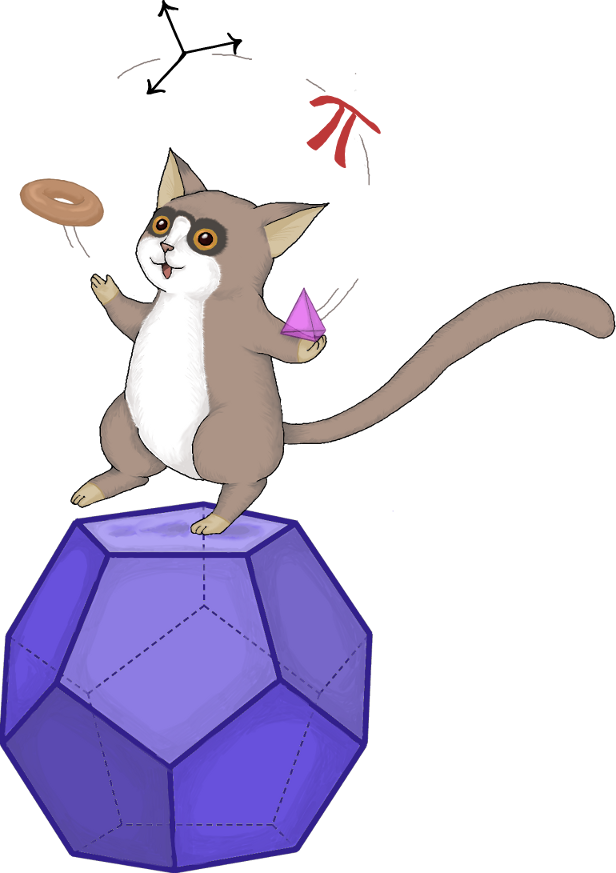
\includegraphics[scale=0.18]{cover}}}

\usepackage{framed}
\definecolor{shadecolor}{rgb}{.97,.97,.97}

\begin{document}

\pagestyle{plain}

\renewcommand{\betreff}{}

%\makeletterhead{}

\vspace{-2em}

\begin{center}
{\qquad\quad}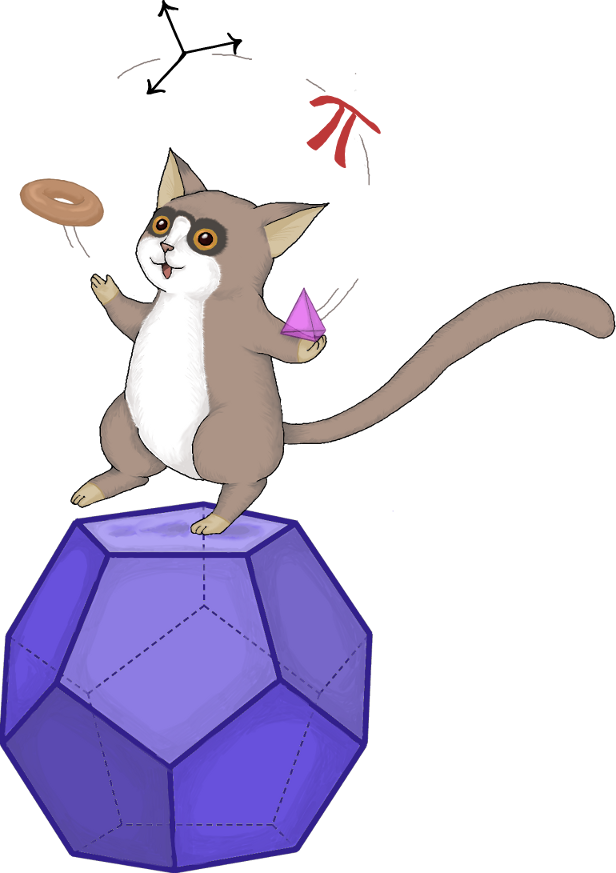
\includegraphics[scale=0.18]{cover}\\[1cm]

  \Large\textbf{\textsf{Bewerbung um den Witty-Jugendförderpreis 2014: \\
  Matheschülerzirkel Augsburg}}
\end{center}

\vspace{1em}

Der Matheschülerzirkel wurde im August~2013 zur Förderung des
Interesses und der Begeisterung für Mathematik unter Schülerinnen und Schülern
an weiterführenden Schulen gegründet. Während des Schuljahrs~2013/2014 betreuen
19~Mitarbeiterinnen und Mitarbeiter ehrenamtlich die knapp
250~teilnehmenden Schülerinnen und Schüler in zweiwöchentlich an der
Universität stattfindenden Präsenzzirkeln. Für weiter entfernt wohnende Schülerinnen
und Schüler unterhalten wir monatliche Korrespondenz per Post.

Als nächstes großes Projekt führen wir ein fünftägiges Mathecamp in den
Sommerferien~2014 durch. Die Angebote des Matheschülerzirkels sind in Augsburg
und Schwaben einzigartig und sollen langfristig weitergeführt und ausgebaut
werden.

\section{Bewerber}

Der Matheschülerzirkel Augsburg ist eine Einrichtung des
Mathematisch-Phy\-si\-ka\-li\-schen Vereins e.V. und wird organisiert von
Mitarbeiterinnen und Mitarbeitern der Universität
Augsburg. Er setzt sich zum Großteil aus Doktorandinnen und Doktoranden,
einigen Professoren und engagierten Studentinnen und Studenten zusammen.

Zu Beginn lief das Projekt als informeller Zusammenschluss von motivierten Doktorandinnen und Doktoranden. Da ein Ziel des Mathematisch-Physikalischen Vereins~e.V. in Augsburg die Darstellung der Mathematik in der Öffentlichkeit ist, fanden wir gemeinsame Interessen und organisieren nun den Matheschülerzirkel im Rahmen des~Vereins.

Die Professorinnen und Professoren des Instituts für Mathematik stehen voll hinter unserem Projekt, der Mathezirkel ist aber eigenständig und keine Einrichtung der Universität Augsburg.

Ein Großteil der Mitwirkenden hat bereits langjährige Erfahrung in
der Jugendarbeit und in der Mathematikbildung. Da einerseits viele junge Zirkelleiterinnen und Zirkelleiter zu unserem Team gehören, können wir
sehr gut mit den Schülerinnen und Schülern kommunizieren.
Andererseits haben wir auch die Unterstützung von erfahrenen Professorinnen und Professoren. Viele von uns nahmen früher selbst an Mathematikzirkeln oder Mathecamps in anderen Regionen teil und wollen nun ihre eigenen prägenden Erfahrungen an die Schülerinnen und Schüler Augsburgs und Schwabens weitergeben.


\begin{center}\small
\renewcommand{\arraystretch}{1.3}
\begin{tabular}{@{}p{5.7cm}@{\qquad}p{6cm}@{\qquad}l@{}}
  \toprule
  \multicolumn{3}{@{}l@{}}{\textbf{Zirkelleiter}} \\
  \toprule
  \textbf{Name} & \textbf{Akademischer Grad} & \textbf{Alter} \\
  Meru Alagalingam & Diplom in Mathematik & 23 \\
 Tim Baumann &  & 20 \\
 Martin Baur & B.\,Sc.\ in Mathematik & 22 \\
 Ingo Blechschmidt & M.\,Sc.\ in Mathematik & 25 \\ 
 Philipp Düren & M.\,Sc.\ in Mathematik & 22 \\ 
 Alexander Engel & M.\,Sc. in Mathematik & 27 \\ 
 Johanna Fleckenstein & M.\,Sc.\ in Mathematik & 26 \\ 
 Kathrin Helmsauer & M.\,Sc.\ in Mathematik & 24 \\ 
 Marco Hien & Prof.\ Dr.\ & 41 \\
 Christian Hübschmann & Diplom in Mathematik & 29 \\ 
 Simon Kapfer & M.\,Sc.\ in Mathematik & 26 \\ 
 Sven Prüfer & M.\,Sc.\ in mathematicher Physik & 27 \\ 
 Peter Quast & Privatdozent, Dr.\ & 38 \\ 
 Lisa Reischmann & M.\,Sc.\ in Mathematik & 23 \\ 
 Peter Uebele & M.\,Sc.\ in mathematicher Physik & 25 \\ 
 Timo Schürg & Prof.\ Dr.\ & 32 \\ 
 Carina Willbold & M.\,Sc.\ in Mathematik & 26 \\ 
 Christopher Wulff & Diplom in Mathematik & 28 \\ 
 Stephanie Zapf & M.\,Sc.\ in Mathematik & 26 \\
\bottomrule
\end{tabular}
\end{center}



\section{Vision}

Unser Ziel ist es, Schülerinnen und Schülern
langfristig eine Möglichkeit zu bieten, ihrem Interesse an der
Mathematik über den Unterricht hinaus nachzugehen. Wir möchten Kinder, die Spaß an der
Mathematik gefunden haben, dazu animieren und darin unterstützen, sich weiter mit der Mathematik zu beschäftigen. Es geht uns darum, diesen Schülerinnen und
Schülern zu zeigen, wie spannend Mathematik sein kann und wie diese außerhalb der Schule aussieht. In diesem Sinne verstehen wir uns als MINT-Förderprojekt.

Im Gegensatz zu anderen Hobbys wie beispielsweise Sport und Musik gibt es für die Mathematik kaum Angebote außerhalb des Schulunterrichts, die nicht der Nachhilfe dienen. Gerade in der Grundschule haben viele Schülerinnen und Schüler eine ausgeprägte Begeisterung für
Rätsel und mathematische Spiele, die leider oft im Laufe der weiteren
Schulzeit verloren geht. Diese Begeisterung möchten wir
durch unser Angebot erhalten und sogar noch ausbauen, indem wir
unseren Teilnehmerinnen und Teilnehmern ermöglichen, sich frei von jeglichem
(Noten-)Druck mathematische Themen zu erarbeiten.

Ein wichtiger Aspekt ist die Vernetzung Gleichgesinnter. An
den meisten weiterführenden Schulen gibt es nur sehr wenige Jugendliche, die sich überdurchschnittlich für Mathematik begeistern. Durch unsere Angebote können die
Schülerinnen und Schüler ihrem Hobby Mathematik gemeinsam in einem motivierenden Umfeld nachgehen.  Viele von uns Mitwirkenden haben selbst als Schüler von derartigen vielfältigen Angeboten profitiert und können aus eigener Erfahrung hervorheben, wie wichtig die so gewonnenen Freundschaften für die persönliche Entwicklung sein können.

Während unsere Kompetenz in der Mathematik liegt und wir daher nur in diesem Bereich Förderprojekte anbieten können, hat unsere Arbeit auch für die anderen MINT-Fächer eine Bedeutung. Schließlich wird Mathematik in allen Naturwissenschaften, der Informatik und der Technik eingesetzt. Jugendlichen, die Spaß an Mathematik haben, steht ein breites Spektrum interessanter Studien- und Berufsmöglichkeiten zur Verfügung. Hier sehen wir auch die Nachhaltigkeit unserer Plattform.

Ein bekanntes Problem im MINT-Bereich ist der niedrige Frauenanteil in Studium und Beruf. Dies ist auch im Bachelor- und Masterstudium der Mathematik zu beobachten. Betrachtet man den hohen Anteil an Studentinnen im Lehramtsstudium, erkennt man, dass offensichtlich ein großes Potenzial zur Erhöhung des Frauenanteils in der Mathematik besteht. Wir richten daher großes Augenmerk darauf, unsere Angebote auch besonders für Schülerinnen ansprechend zu gestalten.

\section{Projektbeschreibung}

Der Matheschülerzirkel Augsburg besteht aus mehreren einander ergänzenden Veranstaltungen, die im
Folgenden einzeln beschrieben werden. Interessierte Schülerinnen und Schüler
können diese unabhängig voneinander besuchen. Bis auf das Mathecamp sind alle
Veranstaltungen für die Teilnehmenden kostenlos.

In Bayrisch-Schwaben gibt es vereinzelte, deutlich kleinere lokale
Projekte, die ähnlich wie wir auf Mathematikförderung bei Schülerinnen und
Schülern ausgerichtet sind. Diese sind aber entweder nur an einzelnen Schulen
angesiedelt und stehen daher nur wenigen Jugendlichen zur Verfügung oder zielen
auf Mathematiknachhilfe ab. Der Matheschülerzirkel Augsburg ist das erste
Projekt in Schwaben, das unabhängig von schulischen Leistungen die
Begeisterung für Mathematik fördern und erhalten möchte.

Unser Projekt grenzt sich deutlich von Nachhilfeangeboten ab, da wir Themen behandeln, die in keiner Schulart auf dem Lehrplan stehen. Somit werden Unterrichtsinhalte weder vorweggenommen noch wiederholt und es handelt sich \emph{nicht} um Nachhilfe.

An anderen Orten wie Leipzig\footnote{\href{http://lsgm.uni-leipzig.de/tiki-index.php}{\textsf{http:/\!/lsgm.uni-leipzig.de/tiki-index.php}}} und Stuttgart\footnote{\href{http://www.mathematik.uni-stuttgart.de/studium/schuelerzirkel/}{\textsf{http:/\!/www.mathematik.uni-stuttgart.de/studium/schuelerzirkel/}}} werden ähnliche Projekte seit
vielen Jahren mit 150 bis 200 Teilnehmenden erfolgreich durchgeführt. Der überwältigende Ansturm in
diesem Schuljahr bei uns zeigte, dass auch hier in Augsburg und Umgebung Nachfrage
besteht.

\subsection{Präsenzzirkel}

Die insgesamt zehn Präsenzzirkel finden in nach Klassenstufe eingeteilten
Kleingruppen von fünf bis zehn Schülerinnen und Schülern statt.
Die jeweilige Gruppe trifft sich nachmittags alle zwei Wochen mit ihrer Zirkelleiterin oder ihrem
Zirkelleiter auf dem Campus der Universität Augsburg und diskutiert und
bearbeitet in gut 90~Minuten Themen der Mathematik, die außerhalb des
Schulstoffs liegen. Durch die kleine Gruppengröße können wir individuell auf
Vorkenntnisse und Themenwünsche eingehen.

Der Ablauf eines Präsenzzirkels hängt stark von der Klassenstufe ab. Bei den
jüngeren Kindern werden Themen eher durch Bearbeiten von passenden
Aufgaben in Eigeninitiative erkundet, während Schülerinnen und Schüler höherer
Klassenstufen auch durch geleitete Diskussionen in der Gruppe
Themen erarbeiten können. In vielen Zirkeln finden spezielle Materialien,
wie zum Beispiel Zauberwürfel, selbstgeschriebene Computerprogramme oder
Bastelutensilien Verwendung.

Die Themen sind sehr vielfältig und reichen unter anderem von
Knobelaufgaben, geheimen Botschaften, Fibonacci-Zahlen und Nim-Spielen (ab Klasse 5),
über Zahlentheorie, Geometrie und Zauberwürfeln (ab Klasse 7) bis hin zu
Fraktalen und Chaos, vierdimensionaler Geometrie und nichtklassischer Logik
(ab Klasse 9). Zusätzlich bieten wir einen Zirkel, der inhaltlich stärker an
mathematischen Wettbewerben ausgerichtet ist.

Die Präsenzzirkel bieten den Teilnehmerinnen und Teilnehmern die Möglichkeit,
gemeinsam mit weiteren mathematisch interessierten Jugendlichen außerhalb der
Schule Mathematik zu betreiben. Im Hinblick auf unser Ziel der Mädchenförderung etablieren wir Zirkelleiterinnen als Vorbilder für die jungen Schülerinnen und vermeiden ungünstige Stereotypen.

Die Zirkel sind für die Schülerinnen und Schüler kostenlos und der Einstieg ist jederzeit möglich.

\subsection{Korrespondenzzirkel}

Viele unserer Schülerinnen und Schüler können aus verschiedenen Gründen
nicht zu unseren Präsenzzirkeln kommen, beispielsweise, weil sie zu weit
entfernt von Augsburg wohnen oder zu viele andere Termine haben.
Daher bieten wir auch schriftliche Korrespondenzzirkel per Post
an.

Wie die Präsenzzirkel sind die Korrespondenzzirkel nach Klassenstufen eingeteilt. Ein
Korrespondenzbrief enthält ein kurzes, von der Zirkelleiterin oder dem
Zirkelleiter geschriebenes Skript zu einem mathematischen Thema sowie passende
Übungsaufgaben. Die Jugendlichen haben pro Brief etwa vier Wochen Zeit, um sich
mit dem Stoff auseinanderzusetzen, die Aufgaben zu lösen und ihre Ergebnisse
an uns zu schicken. Die Zirkelleiterinnen und Zirkelleiter senden dann
ausführliche Korrekturen und Tipps zurück.

Thematisch ähneln sich die beiden Zirkelarten. Genau wie bei den
Präsenzzirkeln ist der Einstieg jederzeit möglich.


\subsection{Mathecamp}

Als drittes großes Projekt führen wir vom 16. bis 20. August erstmals ein fünftägiges
mathematisches Sommercamp durch. Dabei ermöglichen wir bis zu 60~Teilnehmerinnen
und Teilnehmern (je nach unserer finanziellen Lage), sich intensiv mit einer Auswahl mathematischer Themen zu
beschäftigen und Gleichgesinnte kennenzulernen.

Dafür buchten wir das Bruder-Klaus-Heim der Diözese Augsburg in Violau. An jedem Tag beschäftigen sich die Schülerinnen und Schüler in zwei
Arbeitseinheiten mit Themen, die in den Präsenz- und Korrespondenzzirkeln noch
nicht behandelt wurden. Selbstverständlich sind auch diese Kurse nach dem Alter
und den Vorkenntnissen der Teilnehmenden abgestuft. Ferner
werden eine auswärtige Mathematikerin und ein Mathematiker jeweils einen
Vortrag halten.

Für die restliche Zeit bietet unsere Unterkunft ein vielfältiges
Freizeitangebot. Das ist eine besonders gute Gelegenheit für die Jugendlichen,
sich mit ähnlich Interessierten auszutauschen.

Das Camp steht allen mathematisch interessierten Schülerinnen und Schülern der
Klassenstufen~5 bis~12 offen, auch solchen, die unsere anderen Angebote bisher
noch nicht wahrgenommen haben. Wie auch bei unseren sonstigen Veranstaltungen gibt es keine formalen Teilnahmevoraussetzungen. Bei der Vorankündigung stieß das Camp auf großen
Anklang. Die offizielle Anmeldephase begann am 11. Juni 2014.

Schülerinnen und Schüler, die uns erst beim Mathecamp kennenlernen, haben dann die Möglichkeit im neuen Schuljar bei unseren Präsenz- und Korrespondenzzirkeln ihrer Begeisterung für Mathematik zu folgen.

In anderen Regionen werden solche Mathecamps seit vielen Jahren erfolgreich durchgeführt. Jedes Jahr besuchen etwa 100 Jugendliche das Leipziger Mathecamp. Wir sehen daher auch für Augsburg noch großes Steigerungspotenzial, sowohl für die Anzahl der Teilnehmenden als auch die Dauer des Camps.

Als einziges unserer Projekte können wir das Mathecamp nicht kostenlos
anbieten. Wir benötigen eine Eigenbeteiligung von 70~\texteuro{} pro
Teilnehmenden. Die uns tatsächlich entstehenden Kosten liegen bei etwa
200~\texteuro{} pro Kind.

\subsection{Mathematikolympiade}

Im Februar 2015 werden wir auf dem Campus der Universität die Landesrunde der Mathematikolympiade für Schülerinnen und Schüler der Klassenstufen~5 und~6 aus dem Großraum
Augsburg durchführen. Die Mathematikolympiade ist ein internationaler Klausurwettbewerb, deren mehrstufige Auswahlklausuren für die Bundesrunde
bislang dezentral an den einzelnen Schulen durchgeführt wurden. Seit einigen
Jahren gibt es zentrale Landesrunden für die Klassenstufen~7 und höher, die von
\emph{Mathematik-Olympiade in Bayern e.V.} organisiert werden.

Da es aber insbesondere für Schülerinnen und Schüler aus den Klassenstufen~5
und~6 etwas ganz Besonderes ist, für ihre Erfolge in der zweiten Stufe
eingeladen zu werden und die Klausur der Landesrunde gemeinsam mit anderen
Teilnehmerinnen und Teilnehmern zu schreiben, möchten wir diese Veranstaltung
ins Leben rufen.

Dazu laden wir im Februar 2015 ungefähr~50 der in der zweiten Stufe
erfolgreichsten Fünft- und Sechstklässlerinnen und -klässler des Großraums
Augsburg zu uns ein. Diese schreiben dann gemeinsam ihre Olympiadeklausur und
können sich am Nachmittag während der Korrektur unter Betreuung kennenlernen
und austauschen. Abschließend gibt es eine offizielle Siegerehrung.

Eine zentrale Landesrunde ist eine gute Möglichkeit, die sonst von
Hausaufgabenwettbewerben geprägte Mathematikwettbewerbslandschaft durch
Klausurwettbewerbe zu erweitern und dadurch mathematikbegeisterte Schülerinnen
und Schüler zusammenzuführen. Solche für die Schülerinnen und Schüler
sehr besonderen Erfahrungen steigern auch ihr Selbstwertgefühl. Sie zeigen
den Jugendlichen, dass ihre Begeisterung für Mathematik geschätzt wird und dass sie eigenständig Ziele erreichen können.

Wir hoffen, dass sich dadurch auch die Teilnahmequote
in den höheren Klassenstufen langfristig erhöht.


\subsection{Weitere Aktivitäten}

Neben den bereits genannten Zirkeln, dem Mathecamp und der
Matheolympiade organisieren wir noch weitere kleinere
Aktivitäten.

Die wichtigsten zwei Veranstaltungen dieser Art sind die Auftakt- sowie die
Abschlussveranstaltung. Am 09.11.2013 fand unsere erste
Auftaktveranstaltung mit einem anschaulichen und für alle Klassenstufen
geeigneten Vortrag von
Prof.~Dr.~Jost-Hinrich Eschenburg zum Thema \emph{Was sind eigentlich die
Zahlen?} statt.
Die über 150 Teilnehmerinnen und Teilnehmer und deren Eltern waren durchweg
begeistert. Nach einer Stärkung für die Besucher führten wir
die Anmeldung und Terminplanung der Zirkel durch.

Am Ende des Schuljahres wird es eine Abschlussveranstaltung mit einem
weiteren mathematischen Vortrag geben, bei der wir
das vergangene Jahr in den Zirkeln Revue passieren lassen und als Anerkennung
Preise und mathematische Kleingeschenke verteilen. Diese beiden Veranstaltungen sollen
auch in den kommenden Jahren dem Zirkelschuljahr einen Rahmen geben.

Des Weiteren besuchen wir mit unseren Präsenzzirkelteilnehmern die
Vortragsreihe \emph{Faszination Mathematik und Physik}, in welcher viermal im
Jahr Mathematikerinnen und Mathematiker sowie Physikerinnen und Physiker in Augsburg ihre Forschung der
Öffentlichkeit anschaulich darlegen. Außerdem unterstützen wir
Mathematik betreffende Aktionen wie den \emph{Tag der Mathematik} an
der Universität Augsburg oder den \emph{Girl's Day}.

Im kommenden Schuljahr möchten wir Wochenendtreffen für die Teilnehmerinnen und
Teilnehmer der Korrespondenzzirkel anbieten, um auch diesen Jugendlichen die
Möglichkeit zu bieten, sich mit Gleichgesinnten auszutauschen. Diese Treffen
sollen etwa zweimal pro Jahr stattfinden.

Außerdem möchten wir an mehreren Wochenenden einzelne Vorträge in einem
größeren Rahmen anbieten, vorrangig für Schülerinnen und Schüler aus Augsburg.
Die Vorträge sollen von auswärtigen Mathematikerinnen und Mathematikern aus
Wirtschaft und Wissenschaft gehalten werden.


\section{Zielgruppe}

Unser Projekt richtet sich an mathematisch interessierte Schülerinnen
und Schüler der Klassenstufen 5 bis 12. Die einzige Voraussetzung zur
Teilnahme ist Spaß und Interesse an der Mathematik. Es gibt insbesondere
keine Teilnahmebeschränkung durch Noten, Schulzugehörigkeit oder
Wettbewerbsergebnisse.

Im letzten Jahr sahen wir, dass die meisten unserer Kinder eine
sehr hohe Motivation für Mathematik mitbrachten und neugierig auf die
Mathematik außerhalb der Schule waren. Alle Jugendliche, die Interesse an
Rätseln, Logik und abstraktem Denken mitbringen, bilden unsere
Zielgruppe.

Es zeigte sich, dass der Großteil unserer Teilnehmerinnen und
Teilnehmer Gymnasien besucht, aber auch einige Realschülerinnen und "~schüler mitmachen.
Auch Fachoberschülerinnen und "~schülern steht unser Angebot offen, im nächsten
Jahr möchten wir dort verstärkt werben.

Etwa zwei Drittel unserer Teilnehmenden
stammen aus den Klassenstufen~5 bis~8.
Dies deckt sich mit der
Erfahrung an anderen Orten, dass anfangs ein größeres Interesse für
Mathematik besteht und dieses oft im Laufe der Pubertät
deutlich nachlässt -- ein Problem, dem wir gezielt begegnen. Unser Ziel ist, die Schülerinnen und Schüler über ihre gesamte Schullaufbahn hinweg zu begleiten.

Es freut uns sehr, dass 40~Prozent unserer Teilnehmenden weiblich sind. In den Klassenstufen~5 und~6 ist die Quote sogar ausgeglichen. Wir möchten in Zukunft noch mehr Mädchen für den Mathezirkel begeistern.

In den Korrespondenzzirkeln betreuen wir Schülerinnen und Schüler aus ganz
Schwaben, sowie vereinzelt darüber hinaus. Dagegen kommen die Teilnehmerinnen
und Teilnehmer der Präsenzzirkel alle aus dem Großraum Augsburg. Viele davon
nehmen sogar an beiden Zirkeln teil.

\section{Budget}

Wir selbst arbeiten ehrenamtlich. Finanzielle Unterstützung benötigen wir aber
für die von uns durchgeführten Veranstaltungen. Die Professorinnen und
Professoren des Instituts für Mathematik helfen unserem Projekt soweit sie können
und ermöglichen uns, unentgeltlich die Räumlichkeiten der Universität zu nutzen
und organisatorische Ausgaben wie Briefporto über das Institut abzurechnen.
So entstehen uns für die Präsenz- und Korrespondenzzirkel keine Kosten, und
daher können wir diese auch den Schülerinnen und Schülern unentgeltlich
anbieten.

Aus rechtlichen Gründen kann das Institut den Matheschülerzirkel aber leider nicht
direkt finanziell unterstützen, denn wir können weder unter dem Posten
\emph{Lehre} verbucht werden, da unsere Schüler nicht an der Universität
immatrikuliert sind, noch unter dem Posten \emph{Werbung}, da die Zirkel und
das Mathecamp keine Werbeveranstaltungen sein sollen -- obwohl sie natürlich indirekt
durchaus zu einem Aushängeschild der Universität werden können.

Um unser Projekt langfristig durchführen zu können, sind wir daher auf externe
Fördermittel angewiesen.

Auf der nächsten Seite sind in tabellarischer Form unsere geplanten Ausgaben für ein
typisches Schuljahr aufgeführt. Im laufenden Schuljahr konnten wir bis jetzt
neben den Präsenz- und Korrespondenzzirkeln nur die Auftaktveranstaltung
realisieren. Für das in diesem August
stattfindende Mathecamp haben wir über \emph{Bündnis für Augsburg} und ein
Drittmittelprojekt eine einmalige Finanzierungsmöglichkeit gefunden, die
allerdings keine langfristige Option darstellt und nur ein Minimalprogramm mit 40~Teil\-neh\-me\-rin\-nen und Teilnehmern abdeckt. Ohne zusätzliche Finanzierung müssten wir weiteren
Interessenten leider absagen. Außerdem könnten wir einkommensschwache Familien
kaum unterstützen.

Sollten wir den Förderpreis erhalten, wäre die Finanzierung des Mathecamps für dieses Jahr in
voller Höhe gesichert. Außerdem könnten wir sicher unsere für das nächste Schuljahr
geplanten Veranstaltungen durchführen; nur für den vollen Umfang des
Camps~2015 bräuchten wir dann noch zusätzliche Unterstützung. Wir könnten außerdem
eine einmalige Investition in so genannte \emph{dynamische Labyrinthe} tätigen --
das sind etwas teurere Materialien, mit denen man
Computerprogrammierung anschaulich und auch für Schülerinnen und Schüler niedriger Klassenstufen
verständlich erklären kann.

Zur langfristigen Finanzierung stehen wir in Kontakt mit einigen regionalen Firmen und Stiftungen. Mehrere Institutionen zeigten schon Interesse, etwa das bereits erwähnte Bündnis für Augsburg. Manche hatten ihr Budget für dieses Jahr aber schon verplant. Wir sind zuversichtlich, dass wir in den kommenden Jahren mit Blick auf unsere bisherigen Erfolge geeignete Partner finden werden. Darin würde uns der Witty-Jugendförderpreis durch seine Signalwirkung sicher ebenfalls unterstützen.

\begin{center}\small
\renewcommand{\arraystretch}{1.3}
\begin{tabular}{@{}p{5.7cm}@{\qquad}r@{\qquad}p{6cm}@{}}
  \toprule
  \multicolumn{3}{@{}l@{}}{\textbf{Jahresbudget pro Schuljahr}} \\
  \toprule
  \textbf{Auftaktveranstaltung mit 150 Schülern und deren Eltern} & circa 500 \texteuro & im September \\
  {\quad}Verpflegung & 400 \texteuro \\
  {\quad}Flyer und Plakate & 100 \texteuro \\\\
  \textbf{Materialien für Präsenz- und Korrespondenzzirkel} & circa 1.500 \texteuro &
  Bücher zur Kursvorbereitung,
  Bastel- und Anschauungsmaterialien \\\\
  \textbf{Treffen der Korrespondenz\-zirkelteilnehmer} &
  circa $2 \times 300$ \texteuro &
  zwei Mal im Jahr, geplant ab Schuljahr 2014/2015 \\\\
  \textbf{Vortragssamstage} &
  circa $2 \times 300$ \texteuro &
  zwei Mal im Jahr, geplant ab Schuljahr 2014/2015 \\\\
  \textbf{Mathematikolympiade mit 50 Teilnehmern} & circa 1.500 \texteuro &
  im Februar \\\\
  \textbf{Abschlussveranstaltung mit 100 Schülern und deren Eltern} & circa 700 \texteuro &
  im Juli \\
  {\quad}Verpflegung & 300 \texteuro \\
  {\quad}Preise und Urkunden & 400 \texteuro \\\\
  \textbf{Mathecamp \phantom{aaaaaaaaaaaaaa} mit 60 Teilnehmern} & circa 7.300 \texteuro \\
  {\quad}Unterkunft mit Verpflegung & 8.908 \texteuro & 30 \texteuro{} pro Nacht und
  Person zzgl. 11~\texteuro{} Mittagessen am letzten Tag
  (60 Teilnehmer und 8 Betreuer) \\
  {\quad}An- und Abreise & 300 \texteuro & Busunternehmen \\
  {\quad}Versicherung & 330 \texteuro \\
  {\quad}Sonstiges & 1.500 \texteuro & Workshop-Materialien,
  Zwischenmahlzeiten, Freizeitaktivitäten, Benzinkosten eines Autos vor Ort,
  diverse kleinere Posten \\
  {\quad}Eigenbeteiligung & $-$3.800 \texteuro & 70 \texteuro{} pro Kind
  (abzüglich 400 \texteuro{} an Zuschüssen für einkommensschwache Familien) \\
  \bottomrule
  \textbf{Summe} & circa 12.700 \texteuro \\
  \bottomrule
\end{tabular}
\end{center}


\section{Öffentlichkeitsarbeit}

Um auf die Initiierung unseres Projekts zu Beginn des Schuljahrs~2013/2014
aufmerksam zu machen, schickten wir allen Gymnasien Schwabens und einigen
weiteren Schulen im Umkreis von Augsburg Informationspakete mit Lehrerbriefen,
Flyern und Plakaten. Um sicherzugehen, dass unser Angebot in der
Vielzahl der Korrespondenz bei den Schulen nicht unterging, befragten wir außerdem
die Studenten der Universität nach Lehrern, die zu ihrer Schulzeit
besonders großes Engagement zeigten, und schrieben diese separat an.
Häufig zeigten sich diese sehr angetan von unserem Projekt.

Ferner unterstützte uns das Kultusministerium bei der Öffentlichkeitsarbeit, indem es die Schulen direkt zur Beteiligung aufrief.

Schließlich gaben wir eine Pressemitteilung heraus, die von der
Augsburger Allgemeinen aufgegriffen und zu einem prominenten Artikel aufbereitet
wurde (siehe Anlage). Als das Projekt angelaufen war, kam das Augsburger
Regionalfernsehen a.tv auf uns zu und drehte eine kurze Reportage.\footnote{\href{http://www.augsburg.tv/aktuell/schuelerzirkel-mathematik-30_12_2013.html}{\textsf{http:/\!/www.augsburg.tv/aktuell/schuelerzirkel-mathematik-30\_{}12\_{}2013.html}}}

Auf diese Weise konnten wir insgesamt etwa~250 Schülerinnen und Schüler für
unser Projekt begeistern, davon etwa~120 aus dem Großraum Augsburg. Um nun Werbung für
das Mathecamp zu machen, nutzen wir vor allem den bereits etablierten Kontakt
und informieren unsere Schülerinnen und Schüler in den Seminaren persönlich und
zusätzlich per Brief. Ferner verfassen wir wieder eine Pressemitteilung und
benachrichtigen die Augsburger Allgemeine.

Selbstverständlich sind wir auch im Internet auf den Seiten der Universität
vertreten\footnote{\href{http://www.math.uni-augsburg.de/schueler/mathezirkel/}{\textsf{http:/\!/www.math.uni-augsburg.de/schueler/mathezirkel/}}} und schülerfreundlich über Facebook zu erreichen. Über den
Mathematisch-Physikalischen Verein~e.V. erreichen wir Alumni und Freunde der
Universität.


\section{Zeitrahmen}

Die Organisation für den Matheschülerzirkel begann Anfang August~2013. Unsere
erste öffentliche Veranstaltung war die Auftaktveranstaltung am 9. November 2013.
Die Präsenz- und Korrespondenzzirkel sowie
das Sommercamp werden ein fester Bestandteil des Matheschülerzirkels.

Die Korrespondenz- und Präsenzzirkel laufen
das gesamte Schuljahr über. Sie werden von einer
Eröffnungsveranstaltung am Anfang und von einer
Abschlussveranstaltung am Ende des Schuljahres umrahmt. Das Mathecamp soll
einmal jährlich in den Sommerferien stattfinden. Die dritte Stufe der
Matheolympiade für Klassenstufen~5 und~6 findet einmal pro Jahr
im Februar statt und wir planen, diese in
Absprache mit \emph{Mathematik-Olympiade in Bayern e.V.} in Augsburg
durchzuführen.

Das Mathecamp findet vom 16. bis 20.08.2014 statt und wird in den folgenden Jahren ebenfalls in den Sommerferien durchgeführt.

Neben diesen Hauptprojekten möchten wir unseren Schülerinnen und
Schülern weitere Angebote machen, welche ebenfalls permanent angeboten
werden sollen. Dazu gehören Besuche der Vortragsreihe \emph{Faszination
Mathematik und Physik} in Augsburg, Teilnahmen
an Mathematikwettbewerben und mathematischen Schulveranstaltungen der Universität Augsburg.

Da unser Projekt dauerhaft angelegt ist, viele der jetzigen Doktorandinnen und Doktoranden sowie Mitarbeiterinnen und Mitarbeitern in einigen Jahren aber aus der Universität ausscheiden werden,
bemühen wir uns schon jetzt um Verstärkung.
Dazu integrieren wir das Projekt so gut wie möglich mit
dem Institut und dem Verein, sodass auch permanent Beschäftigte,
insbesondere Professorinnen und Professoren, mithelfen. Daneben sprechen wir
aktiv junge Studierende an, um diese auf die Zirkelarbeit
vorzubereiten und zu motivieren, den Matheschülerzirkel
Augsburg in die Zukunft zu führen.


\section{Ansprechpartner}

Die Hauptorganisatoren sind Ingo Blechschmidt, Kathrin Helmsauer und Sven
Prüfer. Sie erreichen uns telefonisch unter 0821/598-5601, 0821/598-5795 bzw.
0821/598-5805. Eine allgemeine E-Mail-Adresse ist
\textsf{mathezirkel@math.uni-augsburg.de}. Unsere persönlichen Adressen sind
\textsf{ingo.blechschmidt@math.uni-augsburg.de},
\textsf{kathrin.helmsauer@""math.uni-augsburg.de} bzw.
\textsf{sven.pruefer@math.uni-augsburg.de}.

Unsere Postanschrift ist:
\vspace{-0.5em}
\begin{tabbing}
  {\qquad} Matheschülerzirkel Augsburg \\
  {\qquad} Lehrstuhl für Algebra und Zahlentheorie \\
  {\qquad} Universitätsstraße 14 \\
  {\qquad} 86159 Augsburg
\end{tabbing}


\section{Erfolgskontrolle}

Unmittelbar und rein qualitativ können wir den Erfolg an den Rückmeldungen der
Kinder und ihrer Eltern messen: Bereitet den Kindern der Präsenzzirkel, der
Korrespondenzzirkel und das Camp Spaß, Freude und Interesse? Gibt es
Verbesserungsvorschläge, Wünsche für das Folgejahr oder anderweitige Kritik?

Quantitativ können wir unseren Erfolg anhand der Teilnehmerzahlen im nächsten
Jahr messen: Wenn den Kindern unsere Veranstaltungen gefallen, werden sie sich
nächstes Jahr wieder anmelden und vielleicht sogar Freunde mitbringen.

Interessant wird auch, zu beobachten, wie sich die Beteiligung an
mathematischen Wettbewerben entwickelt. Wird sich die Zahl der
Teilnehmerinnen und Teilnehmer aus Augsburg und Schwaben am Landeswettbewerb
Mathematik Bayern, am Bundeswettbewerb Mathematik und an der deutschen
Mathematikolympiade durch uns erhöhen? Wir sind bereits erfreut,
dass sich in diesem Jahr vier unserer Teilnehmenden für die
Bundesrunde der Mathematikolympiade qualifizierten.

In unserem ersten Jahr erhielten wir auch schon sehr positive Rückmeldungen der
Kinder und Eltern. Konstruktive Kritik setzen wir im laufenden Betrieb um. Bestätigung der Präsenzzirkel erhielten wir insofern, als dass sie im Laufe des Jahres immer gut besucht blieben.

Verbesserungsmöglichkeiten in den Zirkeln tauschen die Zirkelleiterinnen und -leiter regelmäßig untereinander aus. Für die Zukunft halten wir positive und negative Erfahrungswerte schriftlich fest. Dies erleichtert auch den Austausch mit Mathezirkelprojekten in anderen Regionen. So erreichen wir langfristig eine kontinuierliche Verbesserung unseres Angebot.




\end{document}